% % % % % % % %  MDT UFSM 2021  % % % % % % % % 
%% Arquivo base para o documento - ver. 1.0 %%
% % % % % % % % % % % % % % % % % % % % % % % % 

% % % OPCOES DE COMPILACAO
% % % PAGINACAO
% % % PAGINACAO SIMPLES (FRENTE): PARA TRABALHOS COM MENOS DE 100 PAGINAS
\documentclass[oneside,openright,12pt]{ufsm_2021} %%%%% OPCAO PADRAO -> PAGINACAO SIMPLES. PARA TRABALHOS COM MAIS DE 100 PAGINAS COMENTE ESTA LINHA E DESCOMENTE A LINHA 
% % % % % % % % % % % % % % % % % % % % % % % % % % % % % % % % % % % % % % %
% PAGINACAO DUPLA (FRENTE E VERSO): PARA TRABALHOS COM MAIS DE 100 PAGINAS
% \documentclass[twoside,openright,12pt]{ufsm_2021}  %%%% PARA TRABALHOS COM MAIS DE 100 PAGINAS DESCOMENTE AQUI
% % % % % % % % % % % % % % % % % % % % % % % % % % % % % % % % % % % % %

% % % %  CODIFICACAO DO TEXTO 
% % % %  POR PADRAO USA-SE UTF8. PARA APLICAR A CODIFICACAO OESTE EUROPEU (ISO 8859-1) DESCOMENTE A LINHA ABAIXO. ELA ATIVA A OPCAO "latin1" DO PACOTE "inputenc"
% \oesteeuropeu
% % % % % % % % % % % 

% % % % % % % % PACOTES PESSOAIS % % % % % % % %  
\usepackage{lipsum}
\usepackage{quoting}

% % % % % % % % DEFINICOES PESSOAIS % % % % % % % %

% % % % % % % % % % % % % % % % % % % % % % % % % % % % % % % % % 
% % % % % % % % % % % % DADOS DO TRABALHO % % % % % % % % % % % % 
% % % % % % % % % % % % % % % % % % % % % % % % % % % % % % % % % 

% % % % % % % % % % INFORMACOES INSTITUCIONAIS % % % % % % % % % % 

% % CENTRO DE ENSINO DA UFSM
\centroensino{Centro de Ciências Naturais e Exatas}  %%% NOME POR EXTENSO
\centroensinosigla{CCNE}  %%% SIGLA

% % CURSO DA UFSM
\nivelensino{Pós-Graduação}  %%%%%%% NIVEL DE ENSINO 
\curso{Algum Curso}   %%%%% NOME POR EXTENSO
\ppg{PPGALGO}   %%%%%% SIGLA
\statuscurso{Programa}  %%%% STATUS= {Programa} ou {Curso}
% \EAD  %%%% para cursos EAD
% % % %  LOCAL DO CAMPUS OU POLO
\cidade{Santa Maria}
\estado{RS}


% % % % % % % % % % INFORMACOES DO AUTOR % % % % % % % % % % 
\author{Luan Willig Silveira}   %%%%% AUTOR DO TRABALHO
\sexo{M} %%%% SEXO DO AUTOR -> M=masculino   F=feminino (IMPORTANTE PARA AJUSTAR PAGINAS PRE-TEXTUAIS)
\grauensino{Mestrado}    %%%%%%%% GRAU DE ENSINO A SER CONCLUIDO
\grauobtido{Mestre}    %%%%% TITULO OBTIDO
\email{lalala@uhul.com}   %%%% E-MAIL PARA CATALOGRAFICA (COPYRIGHT) - OBRIGATORIO
% \endereco{Rua das abobrinhas, n. 666} %%%% TELEFONE PARA CATALOGRAFICA (COPYRIGHT) (CAMPO OPICIONAL -- CASO NAO POSSUA OU NAO QUEIRA DIVULGAR COMENTE A LINHA)
% \fone{11 2222 3333}   %%%% TELEFONE PARA CATALOGRAFICA (COPYRIGHT) FORMATO {11 2222 3333} (CAMPO OPICIONAL -- CASO NAO POSSUA OU NAO QUEIRA DIVULGAR COMENTE A LINHA)
% \fax{11 2222 3333}   %%%% FAX PARA CATALOGRAFICA (COPYRIGHT) FORMATO {11 2222 3333} (CAMPO OPICIONAL -- CASO NAO POSSUA OU NAO QUEIRA DIVULGAR COMENTE A LINHA)


% % % % % % % % % % INFORMACOES DA BANCA % % % % % % % % % % 
% OBSERVACOES: O CAMPO ORIENTADOR EH OBRIGATORIO E NAO DEVE SER COMENTADO
% % % % % %    OS DEMAIS MEMBROS DA BANCA (COOREIENTADOR E DEMAIS PROFESSORES) QUANDO COMENTADOS NAO APARECEM NA FOLHA DE APROVACAO (O LAYOUT DA FOLHA DE APROVACAO ESTA PREPARADO PARA O ORIENTADOR E ATE MAIS 4 MEMBROS NA BANCA
\orientador{João da Silva}{Dr}{AAAA}{M}{P}  %%%INFORMACOES SOBRE ORIENTADOR: OS CAMPOS SAO:{NOME}{SIGLA DA TITULACAO}{SIGLA DA INSTITUICAO DE ORIGEM}{SEXO} M=masculino   F=feminino {PARTE DA BANCA?} P=presidente  M=Membro  N=Nao faz parte
\coorientador{Maria da Costa}{Dra}{AAAA}{F}{M} %%%INFORMACOES SOBRE CO-ORIENTADOR: OS CAMPOS SAO:{NOME}{SIGLA DA TITULACAO}{SIGLA DA INSTITUICAO DE ORIGEM}{SEXO} M=masculino   F=feminino {PARTE DA BANCA?} P=presidente  M=Membro  N=Nao faz parte
\bancaum{Banca Um}{Dr}{AAAA}{F}{M}  %%%INFORMACOES SOBRE PRIMEIRO NOME DA BANCA: OS CAMPOS SAO:{NOME}{SIGLA DA TITULACAO}{SIGLA DA INSTITUICAO DE ORIGEM}{SEXO} M=masculino   F=feminino {PARTE DA BANCA?} P=presidente  M=Membro  N=Nao faz parte
%\bancadois{Banca Dois}{Dr}{BBBB}  %%%INFORMACOES SOBRE SEGUNDO NOME DA BANCA: OS CAMPOS SAO:{NOME}{SIGLA DA TITULACAO}{SIGLA DA INSTITUICAO DE ORIGEM}
%\bancatres{Banca Três}{Dra}{CCCC} %%%INFORMACOES SOBRE TERCEIRO NOME DA BANCA: OS CAMPOS SAO:{NOME}{SIGLA DA TITULACAO}{SIGLA DA INSTITUICAO DE ORIGEM}
%\bancaquatro{Banca Quatro}{Dr}{DDDD} %%%INFORMACOES SOBRE QUARTO NOME DA BANCA: OS CAMPOS SAO:{NOME}{SIGLA DA TITULACAO}{SIGLA DA INSTITUICAO DE ORIGEM}
%\bancacinco{Banca Cinco}{Dra}{EEEE} %%%INFORMACOES SOBRE QUARTO NOME DA BANCA: OS CAMPOS SAO:{NOME}{SIGLA DA TITULACAO}{SIGLA DA INSTITUICAO DE ORIGEM}
% \supervisor{Al Paccino}{Dr}{MAFIA}{M}{N} %%%INFORMACOES SOBRE SUPERVISOR (indicado para estagios): OS CAMPOS SAO:{NOME}{SIGLA DA TITULACAO}{SIGLA DA INSTITUICAO DE ORIGEM}{SEXO} M=masculino   F=feminino {PARTE DA BANCA?} P=Presidente  M=Membro  N=Nao faz parte



% % % % % % % % % % REALIZACAO POR VIDEO CONFERENCIA (MEMORANDO 04/2016 BIBLIOTECA CENTRAL UFSM)
\videoconferencia % % % % QUANDO O ACADEMICO DEFENDE POR VIDEO CONFERENCIA (PERMITIDO PELO ARTIGO 82 DO REGIMENTO GERAL DA PRPGP/UFSM). PARA DEFESAS NAS QUAIS O ACADEMICO ESTA PRESENTE COMENTE ESTA LINHA
% % % % QUANDO UM DOS MEMBROS DA BANCA PARTICIPA POR VIDEO CONFERENCIA INDICAR O MEMBRO DE ACORDO COM A LISTA ABAIXO. CASO CONTRARIO MANTER A PALAVRA "NAO". SAO PERMITIDOS, PELO REGIMENTO PRGPGP (ARTIGO 83) ATE 2 MEMBROS 
\videoconferenciabancap{NAO}  %%%% PRIMEIRO MEMBRO
\videoconferenciabancas{NAO}  %%%%% SEGUNDO MEMBRO
% % O > ORIENTADOR
% % CO > COORIENTADOR% % % % QUANDO UM DOS MEMBROS DA BANCA PARTICIPA POR VIDEO CONFERENCIA INDICAR O MEMBRO DE ACORDO COM A LISTA ABAIXO. CASO CONTRARIO MANTER A PALAVRA "NAO". SAO PERMITIDOS, PELO REGIMENTO PRGPGP ATE 2 MEMBROS.
% % 1 > BANCA UM
% % 2 > BANCA DOIS
% % 3 > BANCA TRÊS
% % 4 > BANCA QUATRO
% % 5 > BANCA CINCO
% % S > SUPERVISOR
% % % % % % % % % % % % % % % % % % % % % % % % % % % % % % % % % % % % 



% % % % % % % % % % INFORMACOES SOBRE O TRABALHO % % % % % % % % % %
% % % %  TITULO E SUBTITULO DO TRABALHO: ELES NÃO DEVEM ULTRAPASSAR, JUNTOS, 3 LINHAS NA COMPILAÇÃO DA CAPA. 
% SE O TRABALHO POSSUI SUBTITULO, ADICIONE ':' DENTRO DAS CHAVES ABAIXO 
\titulo{Título do trabalho em português:} %% NAO EH NECESSARIO CAPITALIZAR
% % % %  TITULO DO TRABALHO EM INGLES
% SE O TRABALHO POSSUI SUBTÍTULO, ADICIONE ':' DENTRO DAS CHAVES ABAIXO 
\englishtitle{Título do trabalho em inglês:}  %% NAO EH NECESSARIO CAPITALIZAR


% % % % O SUBTÍTULO É OPCIONAL, SE NÃO FOR USADO AS LINHAS ABAIXO DEVEM SER COMENTADAS

% SE O TRABALHO POSSUI SUBTÍTULO, ADICIONE ':' DENTRO DAS CHAVES ABAIXO 
\subtitulo{Subtítulo do trabalho em português} %% NAO EH NECESSARIO CAPITALIZAR
% % % %  SUB TITULO DO TRABALHO EM INGLES
\subenglishtitle{Subtítulo do trabalho em inglês}  %% NAO EH NECESSARIO CAPITALIZAR

% % % AREA DE CONCENTRACAO DO TRABALHO (CNPQ)
\areaconcentracao{Área de concentração do CNPq}
% % % TIPO DE TRABALHO - MANTER APENAS UMA LINHA DESCOMENTADA
\dissertacao  %% Tese de <nivel de ensino>
% \qualificacao %% Exame de Qualificação de <nivel de ensino>
% \dissertacao %% Dissertacao de <nivel de ensino>
% \monografia %% Monografia
% \monografiag  %% Monografia (nao exibe area de concentracao)
% \tf  %% Trabalho Final de <nivel de ensino>
% \tfg  %% Trabalho Final de Graduacao (nao exibe area de concentracao)
% \tcc  %% Trabalho de Conclusao de Curso
% \tccg  %% Trabalho de Conclusao de Curso (nao exibe area de concentracao)
% \relatorio  %% Relatório de Estágio (nao exibe area de concentracao)
% \generico   %%% Alternativa para aqueles cursos que nao recebem o titulo de bacharel ou licenciado. Ex: engenharia, arquitetura, etc... Os campos abaixo tambem devem ser preenchidos
%     \tipogenerico{Tipo de trabalho em português}
%     \tipogenericoen{Tipo de trabalho em inglês}
%     \concordagenerico{o}
%     \graugenerico{Engenheiro Eletricista}
% % % DATA DA DEFESA 
\data{15}{12}{2011} %% FORMATO {DD}{MM}{AAAA}


% % % % %  RESUMO E PALAVRAS CHAVE DO RESUMO - OBRIGATORIO PARA MDT-UFSM
\resumo{
Escreva seu resumo aqui! Você pode digitá-lo diretamente neste arquivo ou usar o comando input. O resumo deve ter apenas uma página, desde o cabeçalho até as palavras chave. Caso seu resumo seja maior, use comandos para diminuir espaçamento e fonte (até um mínimo de 10pt) no texto.  Segundo a MDT, é preciso que os resumos tenham, no máximo, 250 palavras para trabalhos de conclusão de curso de graduação, pós-graduação e iniciação científica e até 500 palavras para dissertações e teses.
}
\palavrachave{Palavra Chave 1. Palavra 2. Palavra 3. (...)}
% "... deverão constar, no mínimo, três palavras-chave, iniciadas em
% letras maiúsculas, cada termo separado dos demais por ponto, e
% finalizadas também por ponto." MDT 2012

% % % % %  ABSTRACT E PALAVRAS CHAVE DO RESUMO - OBRIGATORIO PARA MDT-UFSM
\abstract{
Write your abstract here! As recomendações do resumo também se aplicam ao abstract. \lipsum[0-1]
}
\keywords{Keyword 1. Keyword 2. Keyword 3. (...)}


% % %  ATIVACAO DE LISTAS E PAGINAS ESPECIAIS
% % %  PARA QUE APARECAO NAO NO TEXTO DESCOMENTE A LINHA ABAIXO -> POR PADRAO TODAS ESTAO ATIVIDADAS

% % LISTA DE FIGURAS 
\semfiguras   %%(QUANDO ATIVIDA NAO EXIBE A LISTA)
% % LISTA DE GRAFICOS 
\semgraficos   %%(QUANDO ATIVIDA NAO EXIBE A LISTA)
% % LISTA DE ILUSTRACOES 
\semilustracoes  %%(QUANDO ATIVIDA NAO EXIBE A LISTA)
% % LISTA DE TABELAS 
\semtabelas   %%(QUANDO ATIVIDA NAO EXIBE A LISTA)
% % LISTA DE QUADROS 
\semquadros   %%(QUANDO ATIVIDA NAO EXIBE A LISTA)
% % LISTA DE APENDICES 
\semapendices  %%(QUANDO ATIVIDA NAO EXIBE A LISTA)
% LISTA DE ANEXOS 
\semanexos   %%(QUANDO ATIVIDA NAO EXIBE A LISTA)


% % % FICHA CATALOGRAFICA
\semcatalografica  %%%%  (QUANDO ATIVIDA NAO EXIBE A FICHA CATALOGRAFICA NECESSITA DO ARQUIVO DA FICHA: ficha_catalografica.pdf
% % % A FICHA CATALOGRAFICA FORNECIDA PELA UFSM EH UM PDF DO TAMANHO A4
% % % EH POSSIVEL GERA-LA NO SITE http://cascavel.ufsm.br/ficha_catalografica/
% % % OS COMANDOS ABAIXO DEFINEM AS MARGENS PARA CORTAR A FICHA FORNECIDA E COLOCA-LA COMO UMA FIGURA NO DOCUMENTO LATEX
\margemesquerda{1.9}   %%%% CORTE DE MARGEM ESQUERDA EM CM
\margemdireita{1.5}   %%%% CORTE DE MARGEM DIREITA EM CM
\margemsuperior{2.75}  %%%% CORTE DE MARGEM SUPERIOR EM CM
\margeminferior{2.9} %%%% CORTE DE MARGEM INFERIOR EM CM
% % %  DICA: IMPRIMA UMA COPIA DA FICHA CATALOGRAFICA E FACA A MEDIDA DAS MARGENS!


% % % % % % % % % % % % % % % % % % % % % % % % % % % % % % % % % % % % % % 
% % % % % % % % % % % %  OPCOES DE FORMATACAO % % % % % % % % % % % % % % %
% % % % % % % % % % % % % % % % % % % % % % % % % % % % % % % % % % % % % % 

% % % % % % % % % % % % % % % % % % % % % % % % % % % % % % % % % % % % % %
% % % FONTES: descomente uma das opcoes. caso nenhuma seja ativada a clase usara a fonte padrao do latex

%% helvetica
\usepackage[scaled]{helvet}
\renewcommand*\familydefault{\sfdefault}

%% arial
% \renewcommand{\rmdefault}{phv} % Arial
% \renewcommand{\sfdefault}{phv} % Arial

%%times
% \usepackage{mathptmx}

\begin{document}

\pretextual

\chapter{Introdução}

\section{Proposta}

O presente estudo tem como objetivo desenvolver uma metodologia capaz de comparar, selecionar, combinar e aprimorar técnicas de processamento de imagem para a detecção e classificação de falhas em isoladores. Para isso, serão estabelecidas métricas para avaliar a eficácia dos processamentos de imagem, considerando aspectos como acurácia e tempo de processamento. Além disso, serão construídos modelos de redes neurais para avaliar o desempenho dos processamentos, podendo abranger tarefas como classificação, detecção e regressão. No decorrer do estudo, serão construídos modelos de redes neurais voltados para a avaliação do desempenho das técnicas de processamento de imagem, sem a intenção de definir um modelo ideal.

Também será analisado o impacto da escolha do modelo de rede neural no desempenho do processamento, visto que diferentes modelos podem gerar resultados distintos para um mesmo processamento. A influência do dataset na eficácia do processamento será outro aspecto a ser investigado, considerando possíveis variações nos resultados devido ao uso de diferentes conjuntos de dados. Para aprimorar os processamentos de imagem, será desenvolvida uma metodologia que permita a combinação de diferentes processamentos unitários (processamentos de imagem que realizam uma única operação). Além disso, será criado um método de ajuste automático de parâmetros das técnicas de processamento de imagem, com o intuito de otimizar seus resultados sem exigir extensa intervenção manual.

A metodologia proposta será desenvolvida dentro de um conjunto de restrições previamente estabelecidas, garantindo um escopo bem delimitado e viável dentro do período de realização da dissertação. Primeiramente, o estudo será restrito à detecção e classificação de falhas em isoladores elétricos, não abrangendo outros componentes elétricos. O uso de imagens previamente adquiridas será uma diretriz, de modo que apenas imagens já disponíveis ou capturadas por métodos convencionais serão utilizadas, sem o desenvolvimento de novas técnicas de aquisição de imagens. Além disso, a metodologia será aplicada exclusivamente a técnicas de processamento de imagem já conhecidas, sem a criação de novos algoritmos de base.

Os modelos de redes neurais desenvolvidos terão o propósito único de avaliar o impacto das redes sobre os processamentos de imagem, sem a intenção de definir um modelo definitivo para diagnóstico industrial. A análise será conduzida utilizando conjuntos de dados já existentes ou obtidos por métodos convencionais, sem a necessidade de criar um novo dataset específico para o estudo. A otimização contemplada estará limitada ao ajuste de parâmetros das técnicas existentes, não incluindo o desenvolvimento de novas abordagens baseadas em inteligência artificial para otimização dos processamentos. Por fim, toda a avaliação será realizada em ambiente controlado, sem a realização de testes em ambientes industriais reais.

A Figura \ref{fig:proposta} ilustra o diagrama da proposta de metodologia.

\begin{figure}[h]
    \centering
    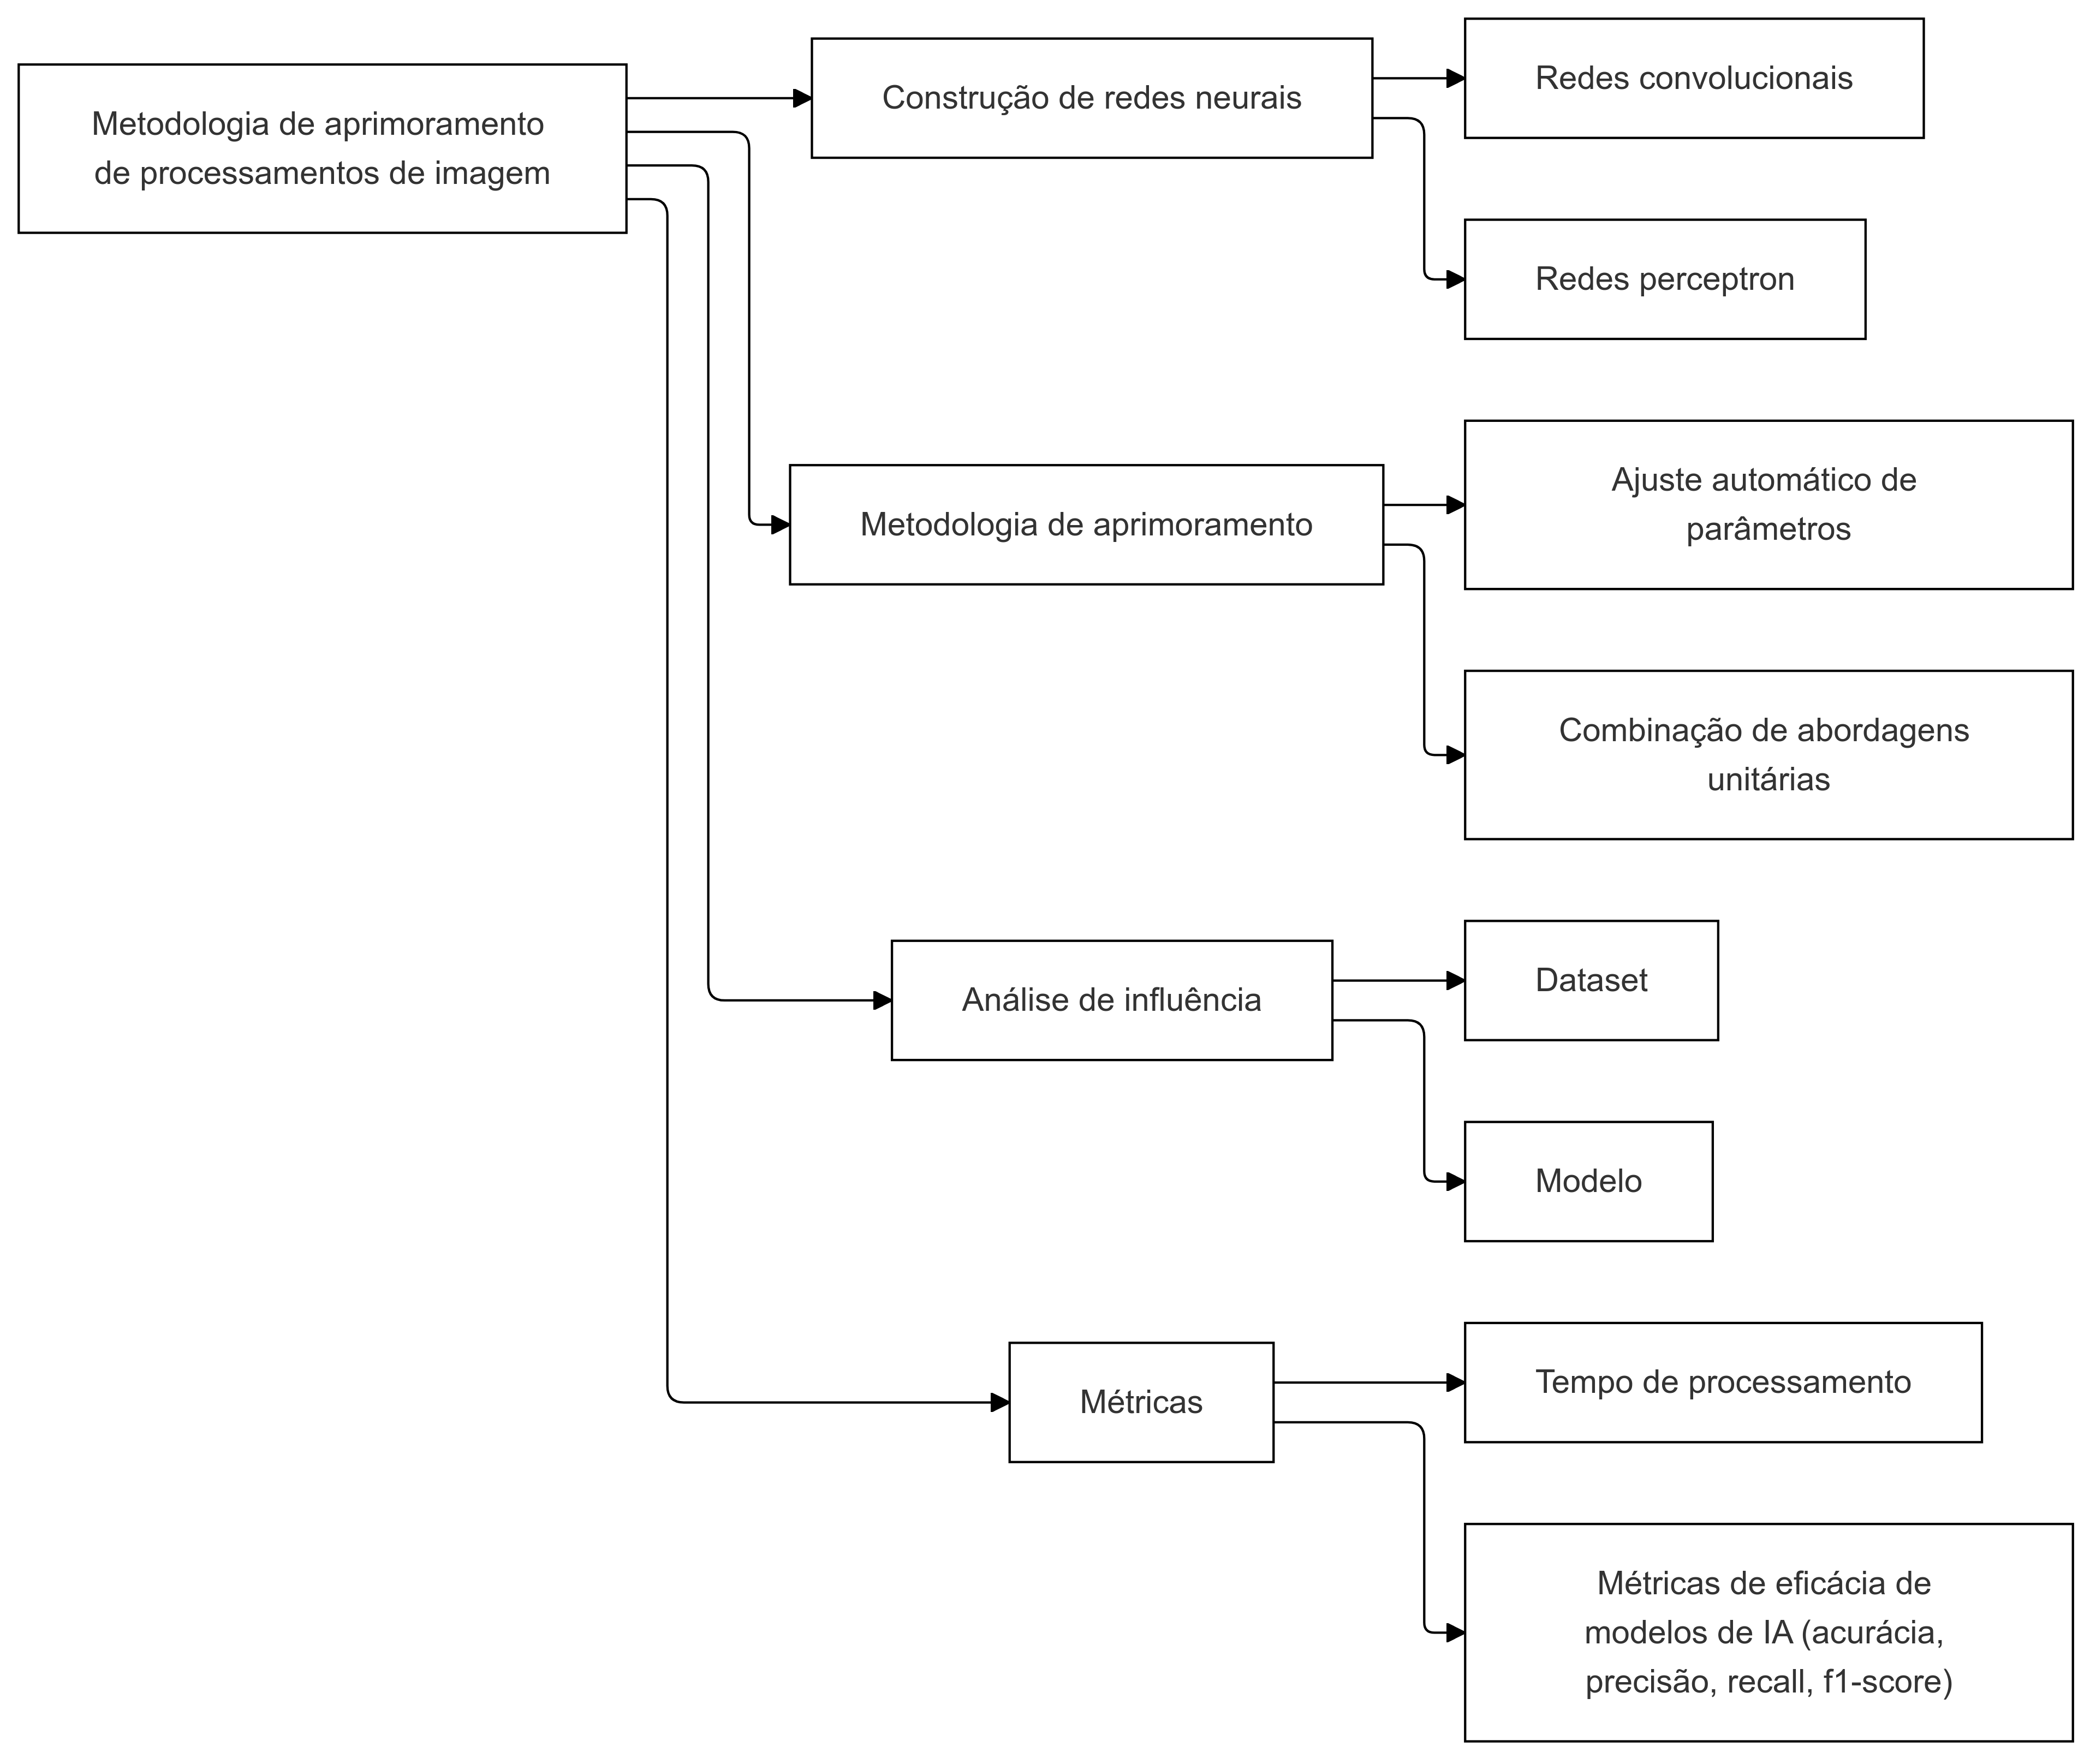
\includegraphics[width=\textwidth]{img/proposta.png}
    \caption{Diagrama da proposta de metodologia}
    \label{fig:proposta}
\end{figure}

\section{Objetivo geral}

O objetivo geral deste estudo é desenvolver uma metodologia capaz de comparar, selecionar, combinar e aprimorar técnicas de processamento de imagem para a detecção e classificação de falhas em isoladores.

\section{Objetivos específicos}

Para alcançar esse objetivo, foram definidos os seguintes objetivos específicos:

\begin{itemize}
    \item Estabelecer métricas para avaliar a eficácia dos processamentos de imagem, considerando aspectos como acurácia e tempo de processamento.
    \item Determinar o tipo de modelo de redes neurais ideal para avaliar o desempenho dos processamentos, podendo abranger classificação, detecção e regressão.
    \item Construir modelos de redes neurais destinados à avaliação do desempenho das técnicas de processamento de imagem, sem o intuito de encontrar um modelo definitivo.
    \item Analisar o impacto da escolha do modelo de rede neural no desempenho do processamento, considerando que diferentes modelos podem gerar diferentes resultados para um mesmo processamento.
    \item Avaliar a influência do dataset na eficácia do processamento, considerando possíveis variações nos resultados devido à utilização de diferentes conjuntos de dados.
    \item Desenvolver uma metodologia para o aprimoramento dos processamentos de imagem por meio da combinação de diferentes abordagens unitárias.
    \item Criar um método de ajuste automático de parâmetros dos processamentos de imagem, visando otimizar seus resultados sem a necessidade de intervenção manual extensa.
\end{itemize}

\section{Justificativa}

A crescente demanda por sistemas automatizados de inspeção de isoladores evidencia a necessidade de técnicas avançadas de processamento de imagem para a detecção precoce de falhas. Conforme demonstrado por Gonzalez e Woods \cite{Gonzalez2008}, a análise digital de imagens permite extrair características relevantes para identificar anomalias em componentes elétricos, possibilitando diagnósticos mais precisos. Ademais, o emprego de redes neurais tem se destacado na resolução de problemas complexos de classificação e detecção, conforme ressaltado por LeCun et al. \cite{LeCun2015} e Krizhevsky et al. \cite{Krizhevsky2012}, contribuindo para a robustez dos sistemas de inspeção.

Estudos recentes apontam que a combinação de diferentes técnicas de processamento de imagem, aliada ao ajuste automático de parâmetros, pode resultar em melhorias significativas no desempenho dos sistemas de diagnóstico \cite{Li2019}. Assim, a proposta deste trabalho visa desenvolver uma metodologia que integre esses avanços, buscando não apenas aprimorar a acurácia e a eficiência dos processamentos, mas também possibilitar uma análise comparativa que leve em conta a influência de diferentes modelos e datasets.

Dessa forma, esta dissertação justifica-se pela necessidade de inovar na abordagem de detecção e classificação de falhas em isoladores, promovendo ganhos práticos para a segurança e manutenção das redes elétricas, e contribuindo para a evolução do estado da arte em processamento de imagem e aprendizado de máquina.

\section{Cronograma}

A seguir, apresenta-se a estrutura das etapas e subetapas que compõem o desenvolvimento deste trabalho. A lista a seguir organiza os principais tópicos a serem abordados ao longo da pesquisa, detalhando desde a introdução até a conclusão, incluindo as metodologias, a revisão bibliográfica, a implementação dos modelos e a análise dos resultados.

\begin{itemize}
    \item \textbf{1. Introdução}
    \begin{itemize}
        \item Justificativa com apresentação do problema e relevância
        \item Objetivos gerais e específicos
        \item Metodologia geral adotada
        \item Estrutura da dissertação
    \end{itemize}
    
    \item \textbf{2. Revisão Bibliográfica}
    \begin{itemize}
        \item Processamento de imagens
        \item Redes neurais para avaliação de processamentos de imagem
        \item Métricas para análise de desempenho (acurácia, tempo, etc.)
        \item Influência de datasets na performance dos modelos
        \item Métodos de ajuste de parâmetros e combinação de processamentos
    \end{itemize}

    \item \textbf{3. Metodologia}
    \begin{itemize}
        \item Definição das métricas para avaliar eficácia dos processamentos
        \item Escolha do tipo de modelo de rede neural (classificação, detecção, regressão, etc.)
        \item Seleção dos datasets para avaliação
        \item Metodologia para combinação de processamentos unitários
        \item Implementação de um método de ajuste automático de parâmetros
    \end{itemize}

    \item \textbf{4. Implementação dos Modelos}
    \begin{itemize}
        \item Construção de redes neurais para avaliação dos processamentos
        \item Testes com diferentes arquiteturas e análise de variações nos resultados
    \end{itemize}

    \item \textbf{5. Análise de Resultados}
    \begin{itemize}
        \item Impacto dos modelos no desempenho dos processamentos
        \item Influência dos datasets nos resultados
        \item Comparação entre diferentes estratégias de processamento
    \end{itemize}

    \item \textbf{6. Conclusão}
    \begin{itemize}
        \item Síntese dos resultados obtidos
        \item Limitações e desafios encontrados
        \item Sugestões para pesquisas futuras
    \end{itemize}
\end{itemize}

A seguir, é apresentado um cronograma de atividades para garantir a organização e a execução das tarefas.

\renewcommand{\arraystretch}{1.5}
\begin{table}[h!]
    \centering
    \resizebox{\textwidth}{!}{
    \begin{tabular}{|l|c|c|c|c|c|c|c|c|c|c|c|}
        \hline
        \textbf{Etapa} & \textbf{Fev} & \textbf{Mar} & \textbf{Abr} & \textbf{Mai} & \textbf{Jun} & \textbf{Jul} & \textbf{Ago} & \textbf{Set} & \textbf{Out} & \textbf{Nov} & \textbf{Dez} \\
        \hline
        \textbf{1. Introdução} & \checkmark &  &  &  &  &  &  &  &  &  &  \\
        \hline
        \textbf{2. Revisão Bibliográfica} & \checkmark & \checkmark & \checkmark & \checkmark & \checkmark &  &  &  &  &  &  \\
        \hline
        \textbf{3. Metodologia} &  & \checkmark & \checkmark & \checkmark & \checkmark & \checkmark & \checkmark &  &  &  &  \\
        \hline
        \textbf{4. Implementação dos Modelos} &  &  &  &  &  & \checkmark & \checkmark &  &  &  &  \\
        \hline
        \textbf{5. Análise de Resultados} &  &  &  &  &  & \checkmark & \checkmark & \checkmark & \checkmark &  &  \\
        \hline
        \textbf{6. Conclusão e Redação Final} &  &  &  &  &  &  &  & \checkmark & \checkmark & \checkmark &  \\
        \hline
        \textbf{7. Defender} &  &  &  &  &  &  &  &  &  &  & \checkmark \\
        \hline
    \end{tabular}}
    \caption{Cronograma de Atividades}
    \label{tab:cronograma}
\end{table}

\chapter{Revisão Bibliográfica}
\section{Processamento de Imagens}
Nesta seção, serão abordados os conceitos fundamentais de processamento de imagens, incluindo técnicas e algoritmos utilizados para a análise e manipulação de imagens digitais. Também será discutida a importância do processamento de imagens no SEP para a detecção e classificação de falhas em equipamentos de linhas de transmissão de energia elétrica.

\section{Datasets}
Será discutida a influência dos datasets na performance dos modelos de processamento de imagem, considerando a importância da escolha de conjuntos de dados representativos e diversificados para o treinamento e avaliação dos modelos.

\section{Redes Neurais}
Aqui, serão discutidos os diferentes tipos de redes neurais aplicáveis ao processamento de imagens, com foco em suas arquiteturas e aplicações específicas para avaliação de desempenho.

\subsection{Métricas}
Serão apresentadas as principais métricas utilizadas para avaliar a eficácia dos processamentos de imagem, como acurácia, tempo de processamento, precisão, recall, entre outras.

\section{Influência de Datasets na Performance dos Modelos}
Esta seção tratará da importância dos datasets na performance dos modelos de processamento de imagem, incluindo a análise de diferentes conjuntos de dados e suas características.

\section{Métodos de Ajuste de Parâmetros e Combinação de Processamentos}
Serão explorados os métodos para ajuste automático de parâmetros e a combinação de diferentes técnicas de processamento de imagem para otimização dos resultados.

\chapter{Metodologia}
\section{Definição das Métricas para Avaliar Eficácia dos Processamentos}
Nesta seção, serão definidas as métricas específicas que serão utilizadas para avaliar a eficácia dos processamentos de imagem no estudo.

\section{Escolha do Tipo de Modelo de Rede Neural}
Será discutida a escolha do tipo de modelo de rede neural mais adequado para as tarefas de classificação, detecção e regressão no contexto do estudo.

\section{Seleção dos Datasets para Avaliação}
Serão apresentados os critérios e a seleção dos datasets que serão utilizados para a avaliação dos processamentos de imagem.

\section{Metodologia para Combinação de Processamentos Unitários}
Aqui, será detalhada a metodologia desenvolvida para combinar diferentes processamentos unitários de imagem visando a melhoria dos resultados.

\section{Implementação de um Método de Ajuste Automático de Parâmetros}
Será descrito o método implementado para ajuste automático de parâmetros das técnicas de processamento de imagem, com o objetivo de otimização sem intervenção manual extensa.

\section{Construção de Redes Neurais para Avaliação dos Processamentos}
Nesta seção, será detalhada a construção dos modelos de redes neurais utilizados para avaliar os processamentos de imagem.

\section{Testes com Diferentes Arquiteturas e Análise de Variações nos Resultados}
Serão apresentados os testes realizados com diferentes arquiteturas de redes neurais e a análise das variações nos resultados obtidos.

\chapter{Análise de Resultados}
\section{Impacto dos Modelos no Desempenho dos Processamentos}
Será analisado o impacto dos diferentes modelos de redes neurais no desempenho dos processamentos de imagem.

\section{Influência dos Datasets nos Resultados}
Aqui, será discutida a influência dos diferentes datasets nos resultados dos processamentos de imagem.

\section{Comparação entre Diferentes Estratégias de Processamento}
Serão comparadas as diferentes estratégias de processamento de imagem utilizadas no estudo, destacando as vantagens e desvantagens de cada uma.

\chapter{Conclusão}
\section{Síntese dos Resultados Obtidos}
Nesta seção, será feita uma síntese dos principais resultados obtidos ao longo do estudo.

\section{Limitações e Desafios Encontrados}
Serão discutidas as limitações e os desafios encontrados durante a realização do trabalho.

\section{Sugestões para Pesquisas Futuras}
Por fim, serão apresentadas sugestões para pesquisas futuras, com base nos resultados e nas limitações identificadas no estudo.

         
\end{document}
